%% LyX 2.3.1-1 created this file.  For more info, see http://www.lyx.org/.
%% Do not edit unless you really know what you are doing.
\documentclass[sigconf,anonymous=true,authordraft=false]{acmart}
\usepackage[latin9]{inputenc}
\usepackage{geometry}
\geometry{verbose,tmargin=0.5cm,bmargin=0.5cm}
\usepackage{float}
\usepackage{graphicx}

\makeatletter
%%%%%%%%%%%%%%%%%%%%%%%%%%%%%% Textclass specific LaTeX commands.
\newlength{\lyxlabelwidth}      % auxiliary length 

%%%%%%%%%%%%%%%%%%%%%%%%%%%%%% User specified LaTeX commands.
%\renewcommand\footnotetextcopyrightpermission[1]{} % removes footnote with conference information in first column
%\pagestyle{plain} % removes running headers


%\makeatletter
%\renewcommand\@formatdoi[1]{\ignorespaces}
%\makeatother


\usepackage{url}
\usepackage{enumitem}
\usepackage{amstext}
\usepackage{graphicx}
\usepackage{booktabs} % For formal tables



\usepackage{subfigure}
\usepackage[ruled,vlined,linesnumbered]{algorithm2e}

\newcommand\varlist{,\makebox[0.8em][c]{.\hfil.\hfil.},} 

% Copyright
%\setcopyright{none}
%\setcopyright{acmcopyright}
%\setcopyright{acmlicensed}
\setcopyright{rightsretained}
%\setcopyright{usgov}
%\setcopyright{usgovmixed}
%\setcopyright{cagov}
%\setcopyright{cagovmixed}


% DOI
\acmDOI{10.475/123_4}

% ISBN
\acmISBN{123-4567-24-567/08/06}

%Conference
\acmConference[WOODSTOCK'97]{ACM Woodstock conference}{July 1997}{El
  Paso, Texas USA} 
\acmYear{1997}
\copyrightyear{2016}

\acmPrice{15.00}

\fancyhead{}
\settopmatter{printacmref=false, printfolios=false}

\makeatother

\begin{document}
\title{An Information Retrieval Perspective of  Filtering for \\Adaptive User Interfaces } 


\newcommand{\subfour}[1]{\vspace*{3mm}{\noindent\bf #1}}  
\newcommand{\subsubfour}[1]{\vspace*{1mm}{\noindent\bf #1}} 
\newtheorem{problem}{\textbf{Problem}}


\section{Celebrity death}

\begin{figure}[H]
\begin{centering}
\subfigure[User Favorites Count.]{\includegraphics[width=0.33\textwidth]{plots_python/Cele_death_user_favouritesCount_boxplots}}\subfigure[User Followers Count.]{\includegraphics[width=0.33\textwidth]{plots_python/Cele_death_user_followersCount_boxplots}}\subfigure[User Friends Count.]{\includegraphics[width=0.33\textwidth]{plots_python/Cele_death_user_friendsCount_boxplots}}
\par\end{centering}
\begin{centering}
\subfigure[User Hashtags Count.]{\includegraphics[width=0.33\textwidth]{plots_python/Cele_death_user_hashtagCount_boxplots}}\subfigure[User Tweets Count.]{\includegraphics[width=0.33\textwidth]{plots_python/Cele_death_user_tweetCount_boxplots}}\subfigure[Hashtag Tweets Count.]{\includegraphics[width=0.33\textwidth]{plots_python/Cele_death_hashtag_tweetCount_boxplots}}
\par\end{centering}
\begin{centering}
\subfigure[Hashtag Users Count.]{\includegraphics[width=0.33\textwidth]{plots_python/Cele_death_hashtag_userCount_boxplots}}\subfigure[Hashtag Users Count.]{\includegraphics[width=0.33\textwidth]{plots_python/Cele_death_location_userCount_boxplots}}\subfigure[Hashtag Users Count.]{\includegraphics[width=0.33\textwidth]{plots_python/Cele_death_mention_tweetCount_boxplots}}
\par\end{centering}
\begin{centering}
\subfigure[Term Users Count.]{\includegraphics[width=0.33\textwidth]{plots_python/Cele_death_term_tweetCount_boxplots}}
\par\end{centering}
\caption{Box-plots for the distribution of Mutual Information values (y-axis)
of different features as a function of their attribute values (binned
on x-axis). }

\end{figure}
\newpage

\begin{figure}[H]
\begin{centering}
\subfigure[User Favorites Count.]{\includegraphics[width=0.33\textwidth]{plots_python/Cele_death_user_favouritesCount_violinplots}}\subfigure[User Followers Count.]{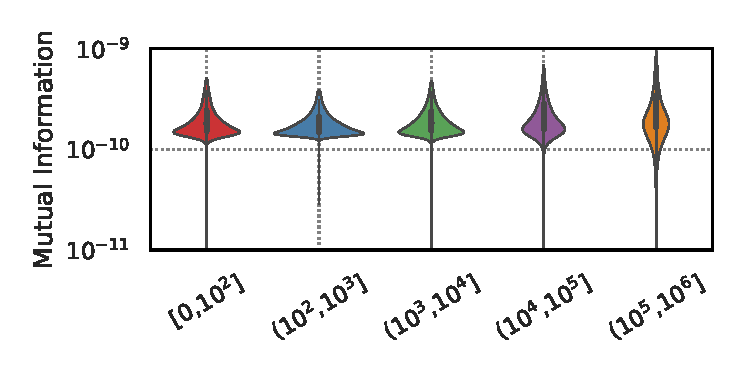
\includegraphics[width=0.33\textwidth]{plots_python/Cele_death_user_followersCount_violinplots}}\subfigure[User Friends Count.]{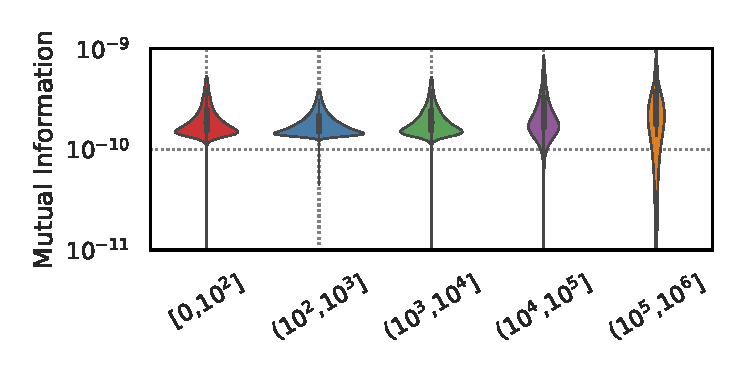
\includegraphics[width=0.33\textwidth]{plots_python/Cele_death_user_friendsCount_violinplots}}
\par\end{centering}
\begin{centering}
\subfigure[User Hashtags Count.]{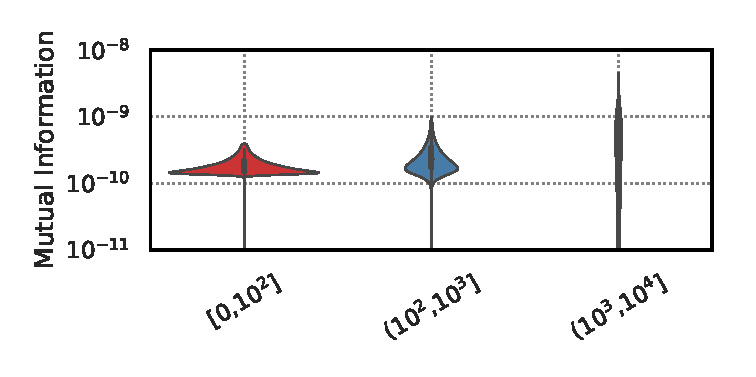
\includegraphics[width=0.33\textwidth]{plots_python/Cele_death_user_hashtagCount_violinplots}}\subfigure[User Tweets Count.]{\includegraphics[width=0.33\textwidth]{plots_python/Cele_death_user_tweetCount_violinplots}}\subfigure[Hashtag Tweets Count.]{\includegraphics[width=0.33\textwidth]{plots_python/Cele_death_hashtag_tweetCount_violinplots}}
\par\end{centering}
\begin{centering}
\subfigure[Hashtag Users Count.]{\includegraphics[width=0.33\textwidth]{plots_python/Cele_death_hashtag_userCount_violinplots}}\subfigure[Hashtag Users Count.]{\includegraphics[width=0.33\textwidth]{plots_python/Cele_death_location_userCount_violinplots}}\subfigure[Hashtag Users Count.]{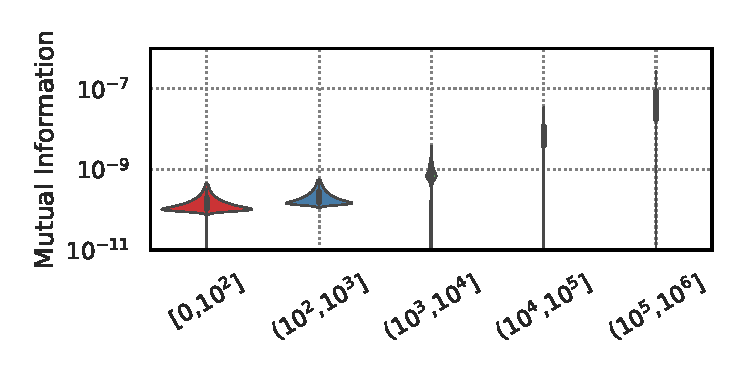
\includegraphics[width=0.33\textwidth]{plots_python/Cele_death_mention_tweetCount_violinplots}}
\par\end{centering}
\begin{centering}
\subfigure[Term Users Count.]{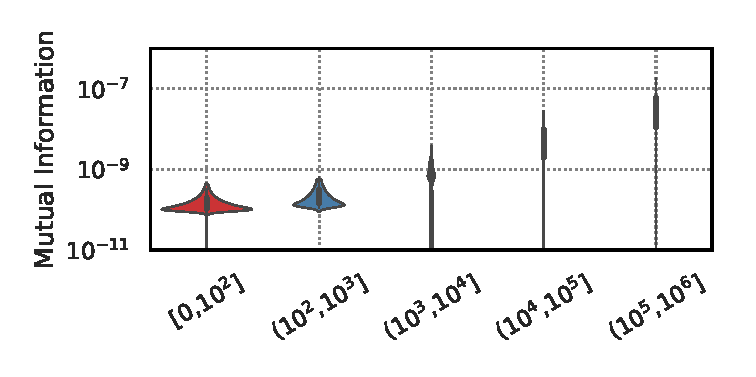
\includegraphics[width=0.33\textwidth]{plots_python/Cele_death_term_tweetCount_violinplots}}
\par\end{centering}
\caption{Violin-plots for the distribution of Mutual Information values (y-axis)
of different features as a function of their attribute values (binned
on x-axis). }

\end{figure}
\newpage

\begin{figure}[H]
\begin{centering}
\subfigure[User Favorites Count.]{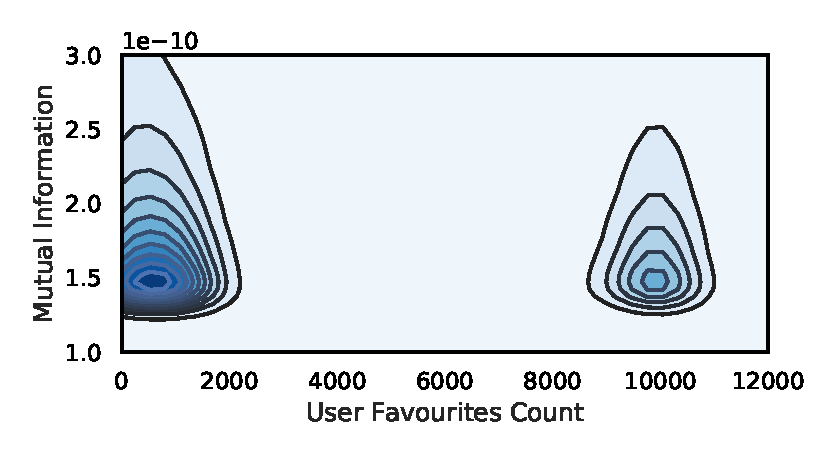
\includegraphics[width=0.33\textwidth]{plots_python/Cele_death_user_favouritesCount_scatter}}\subfigure[User Followers Count.]{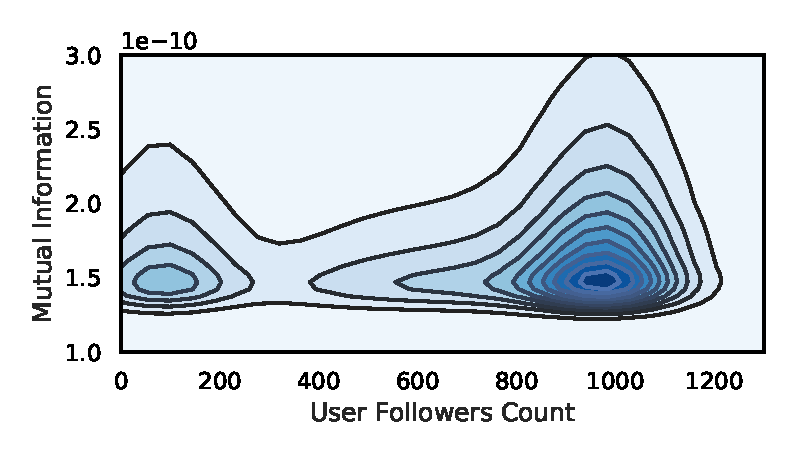
\includegraphics[width=0.33\textwidth]{plots_python/Cele_death_user_followersCount_scatter}}\subfigure[User Friends Count.]{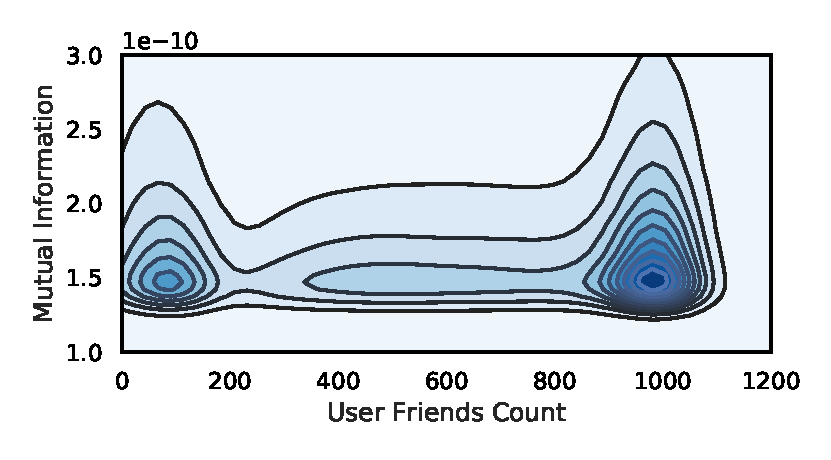
\includegraphics[width=0.33\textwidth]{plots_python/Cele_death_user_friendsCount_scatter}}
\par\end{centering}
\begin{centering}
\subfigure[User Hashtags Count.]{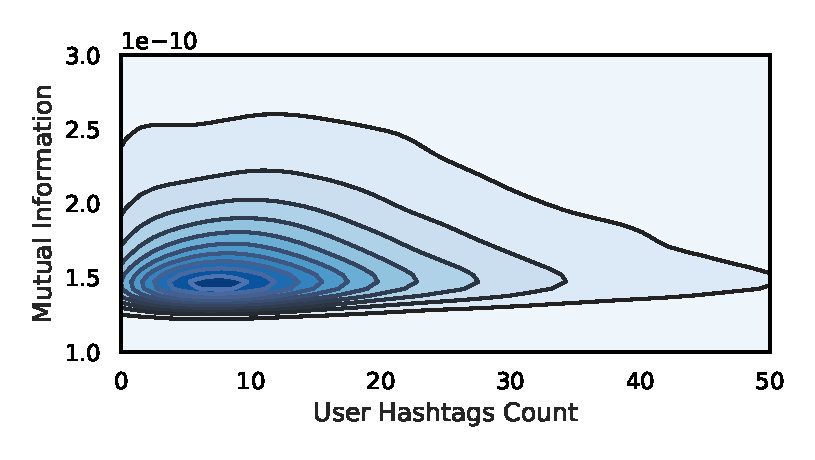
\includegraphics[width=0.33\textwidth]{plots_python/Cele_death_user_hashtagCount_scatter}}\subfigure[User Tweets Count.]{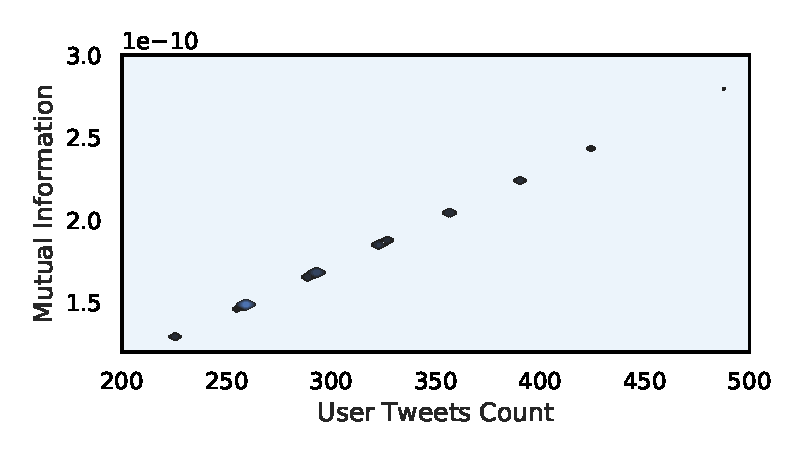
\includegraphics[width=0.33\textwidth]{plots_python/Cele_death_user_tweetCount_scatter}}\subfigure[Hashtag Tweets Count.]{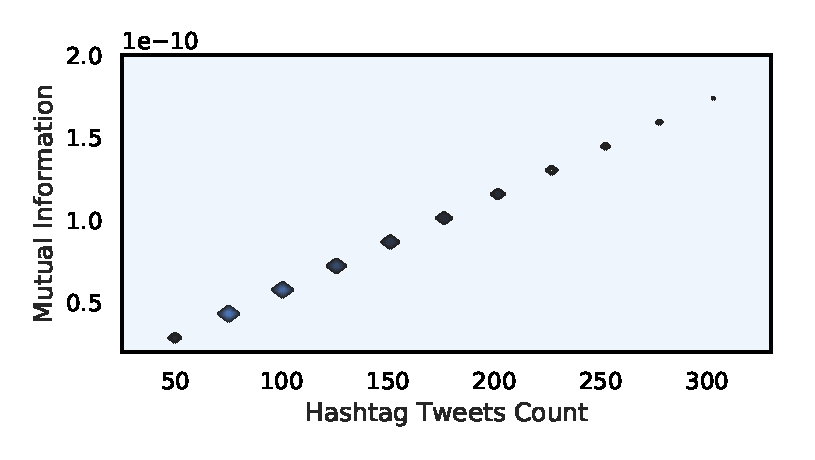
\includegraphics[width=0.33\textwidth]{plots_python/Cele_death_hashtag_tweetCount_scatter}}
\par\end{centering}
\begin{centering}
\subfigure[Hashtag Users Count.]{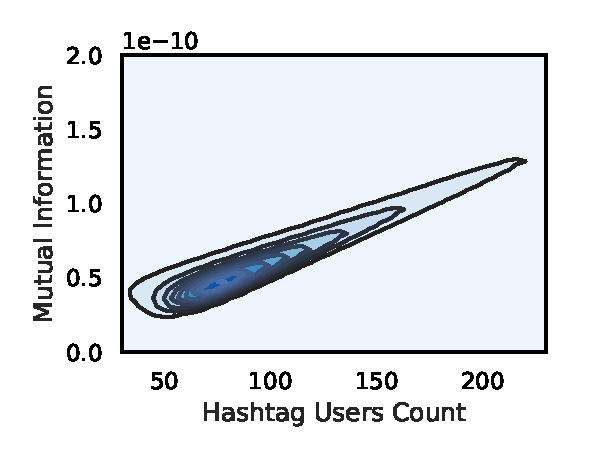
\includegraphics[width=0.33\textwidth]{plots_python/Cele_death_hashtag_userCount_scatter}}\subfigure[Hashtag Users Count.]{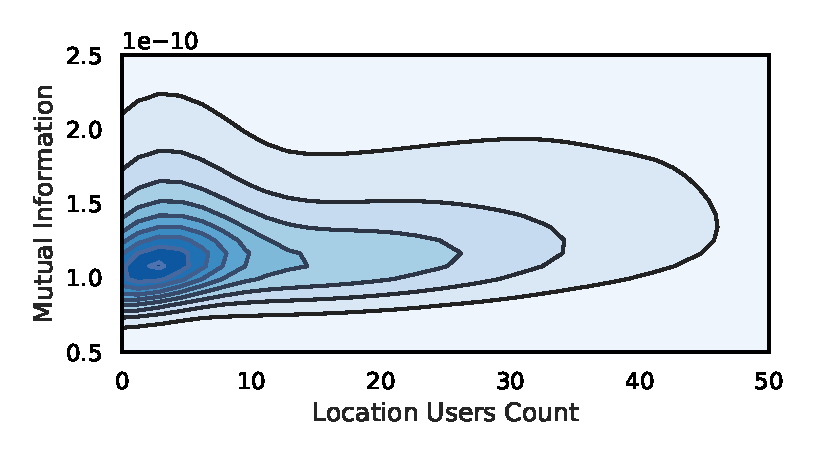
\includegraphics[width=0.33\textwidth]{plots_python/Cele_death_location_userCount_scatter}}\subfigure[Hashtag Users Count.]{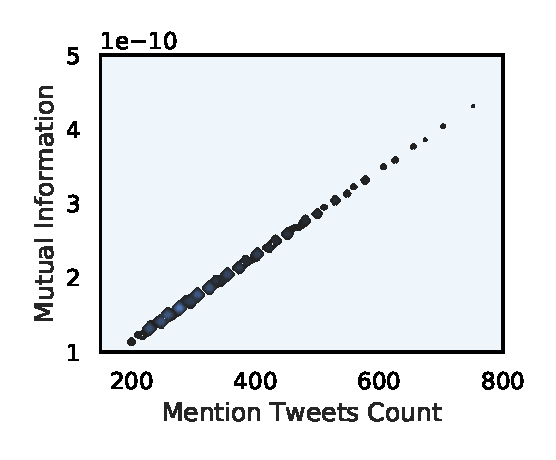
\includegraphics[width=0.33\textwidth]{plots_python/Cele_death_mention_tweetCount_scatter}}
\par\end{centering}
\begin{centering}
\subfigure[Term Users Count.]{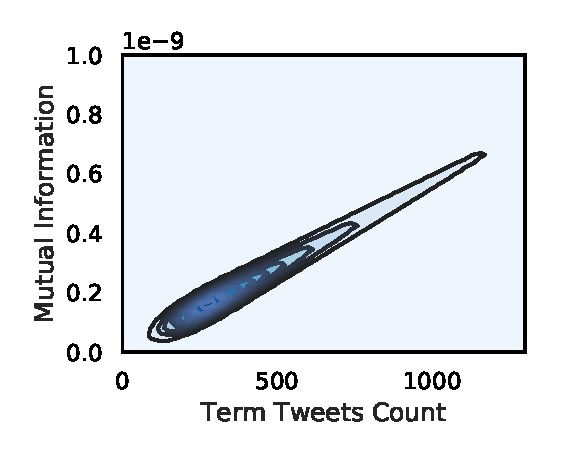
\includegraphics[width=0.33\textwidth]{plots_python/Cele_death_term_tweetCount_scatter}}
\par\end{centering}
\caption{Density plots for the frequency values of feature attributes (x-axis) vs. Mutual Information (y-axis). }

\end{figure}
\newpage

\section{Epidemics}

\begin{figure}[H]
\begin{centering}
\subfigure[User Favorites Count.]{\includegraphics[width=0.33\textwidth]{plots_python/Health_user_favouritesCount_boxplots}}\subfigure[User Followers Count.]{\includegraphics[width=0.33\textwidth]{plots_python/Health_user_followersCount_boxplots}}\subfigure[User Friends Count.]{\includegraphics[width=0.33\textwidth]{plots_python/Health_user_friendsCount_boxplots}}
\par\end{centering}
\begin{centering}
\subfigure[User Hashtags Count.]{\includegraphics[width=0.33\textwidth]{plots_python/Health_user_hashtagCount_boxplots}}\subfigure[User Tweets Count.]{\includegraphics[width=0.33\textwidth]{plots_python/Health_user_tweetCount_boxplots}}\subfigure[Hashtag Tweets Count.]{\includegraphics[width=0.33\textwidth]{plots_python/Health_hashtag_tweetCount_boxplots}}
\par\end{centering}
\begin{centering}
\subfigure[Hashtag Users Count.]{\includegraphics[width=0.33\textwidth]{plots_python/Health_hashtag_userCount_boxplots}}\subfigure[Hashtag Users Count.]{\includegraphics[width=0.33\textwidth]{plots_python/Health_location_userCount_boxplots}}\subfigure[Hashtag Users Count.]{\includegraphics[width=0.33\textwidth]{plots_python/Health_mention_tweetCount_boxplots}}
\par\end{centering}
\begin{centering}
\subfigure[Term Users Count.]{\includegraphics[width=0.33\textwidth]{plots_python/Health_term_tweetCount_boxplots}}
\par\end{centering}
\caption{Box-plots for the distribution of Mutual Information values (y-axis)
of different features as a function of their attribute values (binned
on x-axis). }

\end{figure}
\newpage

\begin{figure}[H]
\begin{centering}
\subfigure[User Favorites Count.]{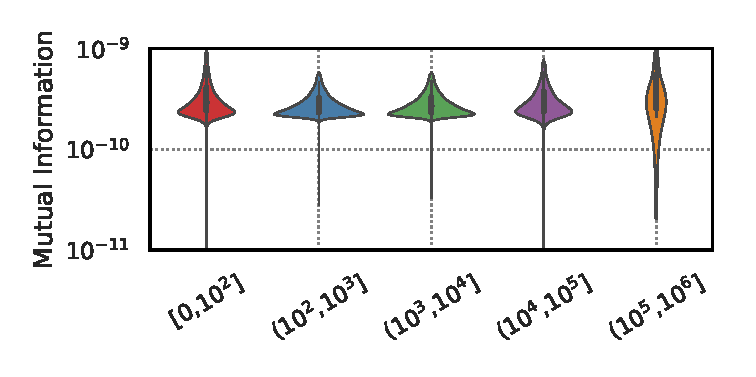
\includegraphics[width=0.33\textwidth]{plots_python/Health_user_favouritesCount_violinplots}}\subfigure[User Followers Count.]{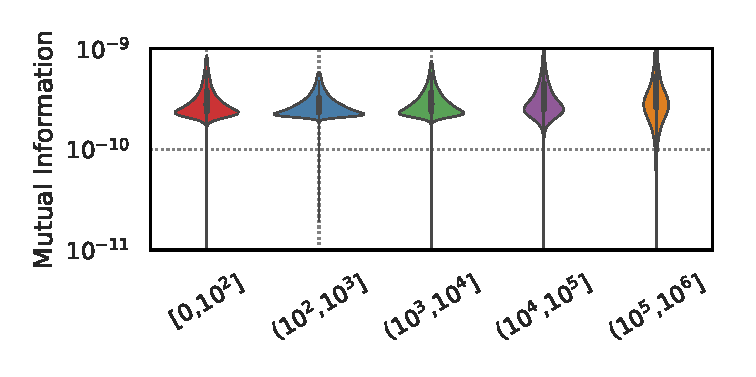
\includegraphics[width=0.33\textwidth]{plots_python/Health_user_followersCount_violinplots}}\subfigure[User Friends Count.]{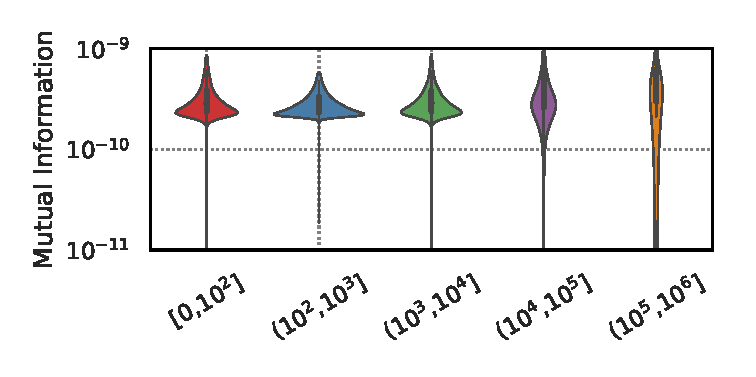
\includegraphics[width=0.33\textwidth]{plots_python/Health_user_friendsCount_violinplots}}
\par\end{centering}
\begin{centering}
\subfigure[User Hashtags Count.]{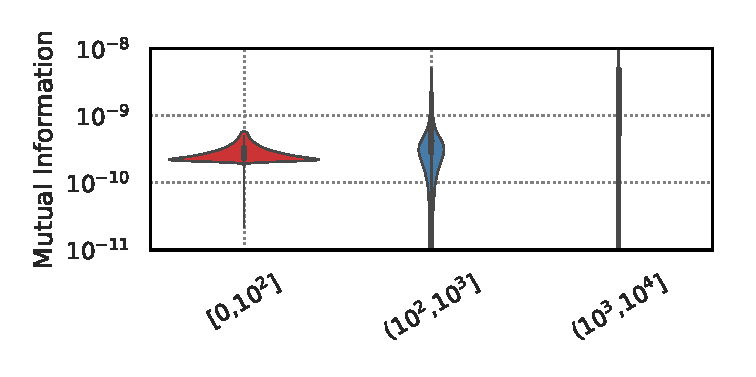
\includegraphics[width=0.33\textwidth]{plots_python/Health_user_hashtagCount_violinplots}}\subfigure[User Tweets Count.]{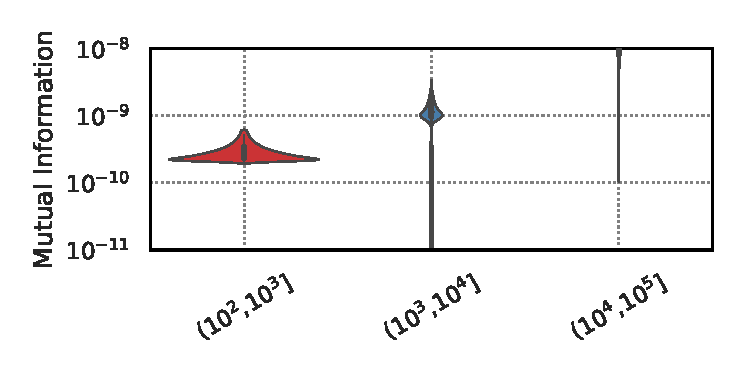
\includegraphics[width=0.33\textwidth]{plots_python/Health_user_tweetCount_violinplots}}\subfigure[Hashtag Tweets Count.]{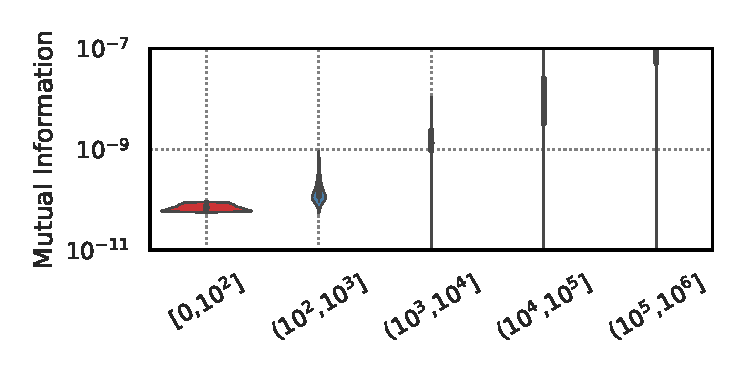
\includegraphics[width=0.33\textwidth]{plots_python/Health_hashtag_tweetCount_violinplots}}
\par\end{centering}
\begin{centering}
\subfigure[Hashtag Users Count.]{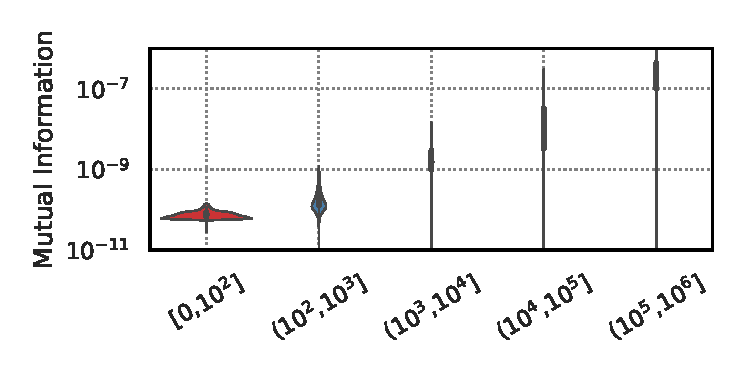
\includegraphics[width=0.33\textwidth]{plots_python/Health_hashtag_userCount_violinplots}}\subfigure[Hashtag Users Count.]{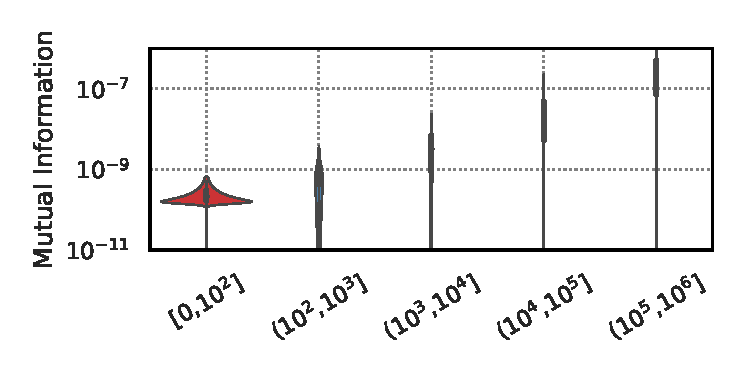
\includegraphics[width=0.33\textwidth]{plots_python/Health_location_userCount_violinplots}}\subfigure[Hashtag Users Count.]{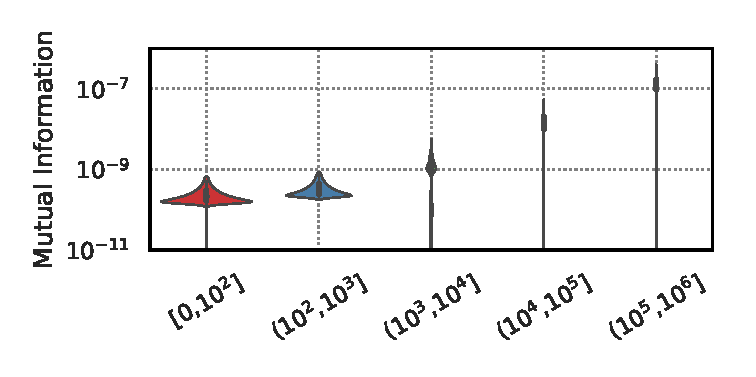
\includegraphics[width=0.33\textwidth]{plots_python/Health_mention_tweetCount_violinplots}}
\par\end{centering}
\begin{centering}
\subfigure[Term Users Count.]{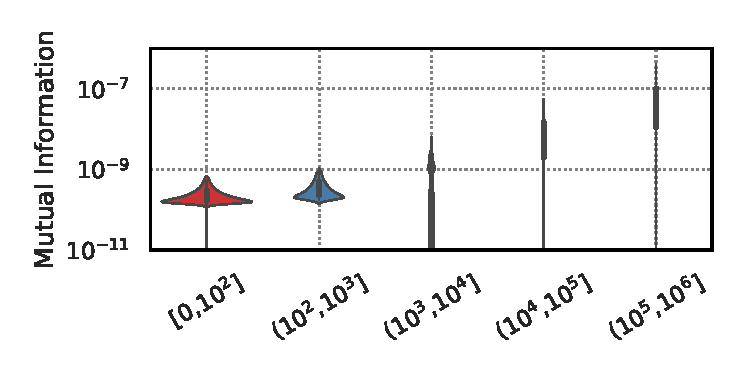
\includegraphics[width=0.33\textwidth]{plots_python/Health_term_tweetCount_violinplots}}
\par\end{centering}
\caption{Violin-plots for the distribution of Mutual Information values (y-axis)
of different features as a function of their attribute values (binned
on x-axis). }

\end{figure}
\newpage

\begin{figure}[H]
\begin{centering}
\subfigure[User Favorites Count.]{\includegraphics[width=0.33\textwidth]{plots_python/Health_user_favouritesCount_scatter}}\subfigure[User Followers Count.]{\includegraphics[width=0.33\textwidth]{plots_python/Health_user_followersCount_scatter}}\subfigure[User Friends Count.]{\includegraphics[width=0.33\textwidth]{plots_python/Health_user_friendsCount_scatter}}
\par\end{centering}
\begin{centering}
\subfigure[User Hashtags Count.]{\includegraphics[width=0.33\textwidth]{plots_python/Health_user_hashtagCount_scatter}}\subfigure[User Tweets Count.]{\includegraphics[width=0.33\textwidth]{plots_python/Health_user_tweetCount_scatter}}\subfigure[Hashtag Tweets Count.]{\includegraphics[width=0.33\textwidth]{plots_python/Health_hashtag_tweetCount_scatter}}
\par\end{centering}
\begin{centering}
\subfigure[Hashtag Users Count.]{\includegraphics[width=0.33\textwidth]{plots_python/Health_hashtag_userCount_scatter}}\subfigure[Hashtag Users Count.]{\includegraphics[width=0.33\textwidth]{plots_python/Health_location_userCount_scatter}}\subfigure[Hashtag Users Count.]{\includegraphics[width=0.33\textwidth]{plots_python/Health_mention_tweetCount_scatter}}
\par\end{centering}
\begin{centering}
\subfigure[Term Users Count.]{\includegraphics[width=0.33\textwidth]{plots_python/Health_term_tweetCount_scatter}}
\par\end{centering}
\caption{Density plots for the frequency values of feature attributes (x-axis) vs. Mutual Information (y-axis). }

\end{figure}
\newpage

\section{Human Disaster}


\begin{figure}[H]
\begin{centering}
\subfigure[User Favorites Count.]{\includegraphics[width=0.33\textwidth]{plots_python/Human_Disaster_user_favouritesCount_boxplots}}\subfigure[User Followers Count.]{\includegraphics[width=0.33\textwidth]{plots_python/Human_Disaster_user_followersCount_boxplots}}\subfigure[User Friends Count.]{\includegraphics[width=0.33\textwidth]{plots_python/Human_Disaster_user_friendsCount_boxplots}}
\par\end{centering}
\begin{centering}
\subfigure[User Hashtags Count.]{\includegraphics[width=0.33\textwidth]{plots_python/Human_Disaster_user_hashtagCount_boxplots}}\subfigure[User Tweets Count.]{\includegraphics[width=0.33\textwidth]{plots_python/Human_Disaster_user_tweetCount_boxplots}}\subfigure[Hashtag Tweets Count.]{\includegraphics[width=0.33\textwidth]{plots_python/Human_Disaster_hashtag_tweetCount_boxplots}}
\par\end{centering}
\begin{centering}
\subfigure[Hashtag Users Count.]{\includegraphics[width=0.33\textwidth]{plots_python/Human_Disaster_hashtag_userCount_boxplots}}\subfigure[Hashtag Users Count.]{\includegraphics[width=0.33\textwidth]{plots_python/Human_Disaster_location_userCount_boxplots}}\subfigure[Hashtag Users Count.]{\includegraphics[width=0.33\textwidth]{plots_python/Human_Disaster_mention_tweetCount_boxplots}}
\par\end{centering}
\begin{centering}
\subfigure[Term Users Count.]{\includegraphics[width=0.33\textwidth]{plots_python/Human_Disaster_term_tweetCount_boxplots}}
\par\end{centering}
\caption{Box-plots for the distribution of Mutual Information values (y-axis)
of different features as a function of their attribute values (binned
on x-axis). }

\end{figure}
\newpage

\begin{figure}[H]
\begin{centering}
\subfigure[User Favorites Count.]{\includegraphics[width=0.33\textwidth]{plots_python/Human_Disaster_user_favouritesCount_violinplots}}\subfigure[User Followers Count.]{\includegraphics[width=0.33\textwidth]{plots_python/Human_Disaster_user_followersCount_violinplots}}\subfigure[User Friends Count.]{\includegraphics[width=0.33\textwidth]{plots_python/Human_Disaster_user_friendsCount_violinplots}}
\par\end{centering}
\begin{centering}
\subfigure[User Hashtags Count.]{\includegraphics[width=0.33\textwidth]{plots_python/Human_Disaster_user_hashtagCount_violinplots}}\subfigure[User Tweets Count.]{\includegraphics[width=0.33\textwidth]{plots_python/Human_Disaster_user_tweetCount_violinplots}}\subfigure[Hashtag Tweets Count.]{\includegraphics[width=0.33\textwidth]{plots_python/Human_Disaster_hashtag_tweetCount_violinplots}}
\par\end{centering}
\begin{centering}
\subfigure[Hashtag Users Count.]{\includegraphics[width=0.33\textwidth]{plots_python/Human_Disaster_hashtag_userCount_violinplots}}\subfigure[Hashtag Users Count.]{\includegraphics[width=0.33\textwidth]{plots_python/Human_Disaster_location_userCount_violinplots}}\subfigure[Hashtag Users Count.]{\includegraphics[width=0.33\textwidth]{plots_python/Human_Disaster_mention_tweetCount_violinplots}}
\par\end{centering}
\begin{centering}
\subfigure[Term Users Count.]{\includegraphics[width=0.33\textwidth]{plots_python/Human_Disaster_term_tweetCount_violinplots}}
\par\end{centering}
\caption{Violin-plots for the distribution of Mutual Information values (y-axis)
of different features as a function of their attribute values (binned
on x-axis). }

\end{figure}
\newpage

\begin{figure}[H]
\begin{centering}
\subfigure[User Favorites Count.]{\includegraphics[width=0.33\textwidth]{plots_python/Human_Disaster_user_favouritesCount_scatter}}\subfigure[User Followers Count.]{\includegraphics[width=0.33\textwidth]{plots_python/Human_Disaster_user_followersCount_scatter}}\subfigure[User Friends Count.]{\includegraphics[width=0.33\textwidth]{plots_python/Human_Disaster_user_friendsCount_scatter}}
\par\end{centering}
\begin{centering}
\subfigure[User Hashtags Count.]{\includegraphics[width=0.33\textwidth]{plots_python/Human_Disaster_user_hashtagCount_scatter}}\subfigure[User Tweets Count.]{\includegraphics[width=0.33\textwidth]{plots_python/Human_Disaster_user_tweetCount_scatter}}\subfigure[Hashtag Tweets Count.]{\includegraphics[width=0.33\textwidth]{plots_python/Human_Disaster_hashtag_tweetCount_scatter}}
\par\end{centering}
\begin{centering}
\subfigure[Hashtag Users Count.]{\includegraphics[width=0.33\textwidth]{plots_python/Human_Disaster_hashtag_userCount_scatter}}\subfigure[Hashtag Users Count.]{\includegraphics[width=0.33\textwidth]{plots_python/Human_Disaster_location_userCount_scatter}}\subfigure[Hashtag Users Count.]{\includegraphics[width=0.33\textwidth]{plots_python/Human_Disaster_mention_tweetCount_scatter}}
\par\end{centering}
\begin{centering}
\subfigure[Term Users Count.]{\includegraphics[width=0.33\textwidth]{plots_python/Human_Disaster_term_tweetCount_scatter}}
\par\end{centering}
\caption{Density plots for the frequency values of feature attributes (x-axis) vs. Mutual Information (y-axis). }

\end{figure}
\newpage

\section{Iean Nuclear Deal}


\begin{figure}[H]
\begin{centering}
\subfigure[User Favorites Count.]{\includegraphics[width=0.33\textwidth]{plots_python/Iran_user_favouritesCount_boxplots}}\subfigure[User Followers Count.]{\includegraphics[width=0.33\textwidth]{plots_python/Iran_user_followersCount_boxplots}}\subfigure[User Friends Count.]{\includegraphics[width=0.33\textwidth]{plots_python/Iran_user_friendsCount_boxplots}}
\par\end{centering}
\begin{centering}
\subfigure[User Hashtags Count.]{\includegraphics[width=0.33\textwidth]{plots_python/Iran_user_hashtagCount_boxplots}}\subfigure[User Tweets Count.]{\includegraphics[width=0.33\textwidth]{plots_python/Iran_user_tweetCount_boxplots}}\subfigure[Hashtag Tweets Count.]{\includegraphics[width=0.33\textwidth]{plots_python/Iran_hashtag_tweetCount_boxplots}}
\par\end{centering}
\begin{centering}
\subfigure[Hashtag Users Count.]{\includegraphics[width=0.33\textwidth]{plots_python/Iran_hashtag_userCount_boxplots}}\subfigure[Hashtag Users Count.]{\includegraphics[width=0.33\textwidth]{plots_python/Iran_location_userCount_boxplots}}\subfigure[Hashtag Users Count.]{\includegraphics[width=0.33\textwidth]{plots_python/Iran_mention_tweetCount_boxplots}}
\par\end{centering}
\begin{centering}
\subfigure[Term Users Count.]{\includegraphics[width=0.33\textwidth]{plots_python/Iran_term_tweetCount_boxplots}}
\par\end{centering}
\caption{Box-plots for the distribution of Mutual Information values (y-axis)
of different features as a function of their attribute values (binned
on x-axis). }

\end{figure}
\newpage

\begin{figure}[H]
\begin{centering}
\subfigure[User Favorites Count.]{\includegraphics[width=0.33\textwidth]{plots_python/Iran_user_favouritesCount_violinplots}}\subfigure[User Followers Count.]{\includegraphics[width=0.33\textwidth]{plots_python/Iran_user_followersCount_violinplots}}\subfigure[User Friends Count.]{\includegraphics[width=0.33\textwidth]{plots_python/Iran_user_friendsCount_violinplots}}
\par\end{centering}
\begin{centering}
\subfigure[User Hashtags Count.]{\includegraphics[width=0.33\textwidth]{plots_python/Iran_user_hashtagCount_violinplots}}\subfigure[User Tweets Count.]{\includegraphics[width=0.33\textwidth]{plots_python/Iran_user_tweetCount_violinplots}}\subfigure[Hashtag Tweets Count.]{\includegraphics[width=0.33\textwidth]{plots_python/Iran_hashtag_tweetCount_violinplots}}
\par\end{centering}
\begin{centering}
\subfigure[Hashtag Users Count.]{\includegraphics[width=0.33\textwidth]{plots_python/Iran_hashtag_userCount_violinplots}}\subfigure[Hashtag Users Count.]{\includegraphics[width=0.33\textwidth]{plots_python/Iran_location_userCount_violinplots}}\subfigure[Hashtag Users Count.]{\includegraphics[width=0.33\textwidth]{plots_python/Iran_mention_tweetCount_violinplots}}
\par\end{centering}
\begin{centering}
\subfigure[Term Users Count.]{\includegraphics[width=0.33\textwidth]{plots_python/Iran_term_tweetCount_violinplots}}
\par\end{centering}
\caption{Violin-plots for the distribution of Mutual Information values (y-axis)
of different features as a function of their attribute values (binned
on x-axis). }

\end{figure}
\newpage

\begin{figure}[H]
\begin{centering}
\subfigure[User Favorites Count.]{\includegraphics[width=0.33\textwidth]{plots_python/Iran_user_favouritesCount_scatter}}\subfigure[User Followers Count.]{\includegraphics[width=0.33\textwidth]{plots_python/Iran_user_followersCount_scatter}}\subfigure[User Friends Count.]{\includegraphics[width=0.33\textwidth]{plots_python/Iran_user_friendsCount_scatter}}
\par\end{centering}
\begin{centering}
\subfigure[User Hashtags Count.]{\includegraphics[width=0.33\textwidth]{plots_python/Iran_user_hashtagCount_scatter}}\subfigure[User Tweets Count.]{\includegraphics[width=0.33\textwidth]{plots_python/Iran_user_tweetCount_scatter}}\subfigure[Hashtag Tweets Count.]{\includegraphics[width=0.33\textwidth]{plots_python/Iran_hashtag_tweetCount_scatter}}
\par\end{centering}
\begin{centering}
\subfigure[Hashtag Users Count.]{\includegraphics[width=0.33\textwidth]{plots_python/Iran_hashtag_userCount_scatter}}\subfigure[Hashtag Users Count.]{\includegraphics[width=0.33\textwidth]{plots_python/Iran_location_userCount_scatter}}\subfigure[Hashtag Users Count.]{\includegraphics[width=0.33\textwidth]{plots_python/Iran_mention_tweetCount_scatter}}
\par\end{centering}
\begin{centering}
\subfigure[Term Users Count.]{\includegraphics[width=0.33\textwidth]{plots_python/Iran_term_tweetCount_scatter}}
\par\end{centering}
\caption{Density plots for the frequency values of feature attributes (x-axis) vs. Mutual Information (y-axis). }

\end{figure}
\newpage


\section{LGBT}


\begin{figure}[H]
\begin{centering}
\subfigure[User Favorites Count.]{\includegraphics[width=0.33\textwidth]{plots_python/LGBT_user_favouritesCount_boxplots}}\subfigure[User Followers Count.]{\includegraphics[width=0.33\textwidth]{plots_python/LGBT_user_followersCount_boxplots}}\subfigure[User Friends Count.]{\includegraphics[width=0.33\textwidth]{plots_python/LGBT_user_friendsCount_boxplots}}
\par\end{centering}
\begin{centering}
\subfigure[User Hashtags Count.]{\includegraphics[width=0.33\textwidth]{plots_python/LGBT_user_hashtagCount_boxplots}}\subfigure[User Tweets Count.]{\includegraphics[width=0.33\textwidth]{plots_python/LGBT_user_tweetCount_boxplots}}\subfigure[Hashtag Tweets Count.]{\includegraphics[width=0.33\textwidth]{plots_python/LGBT_hashtag_tweetCount_boxplots}}
\par\end{centering}
\begin{centering}
\subfigure[Hashtag Users Count.]{\includegraphics[width=0.33\textwidth]{plots_python/LGBT_hashtag_userCount_boxplots}}\subfigure[Hashtag Users Count.]{\includegraphics[width=0.33\textwidth]{plots_python/LGBT_location_userCount_boxplots}}\subfigure[Hashtag Users Count.]{\includegraphics[width=0.33\textwidth]{plots_python/LGBT_mention_tweetCount_boxplots}}
\par\end{centering}
\begin{centering}
\subfigure[Term Users Count.]{\includegraphics[width=0.33\textwidth]{plots_python/LGBT_term_tweetCount_boxplots}}
\par\end{centering}
\caption{Box-plots for the distribution of Mutual Information values (y-axis)
of different features as a function of their attribute values (binned
on x-axis). }

\end{figure}
\newpage

\begin{figure}[H]
\begin{centering}
\subfigure[User Favorites Count.]{\includegraphics[width=0.33\textwidth]{plots_python/LGBT_user_favouritesCount_violinplots}}\subfigure[User Followers Count.]{\includegraphics[width=0.33\textwidth]{plots_python/LGBT_user_followersCount_violinplots}}\subfigure[User Friends Count.]{\includegraphics[width=0.33\textwidth]{plots_python/LGBT_user_friendsCount_violinplots}}
\par\end{centering}
\begin{centering}
\subfigure[User Hashtags Count.]{\includegraphics[width=0.33\textwidth]{plots_python/LGBT_user_hashtagCount_violinplots}}\subfigure[User Tweets Count.]{\includegraphics[width=0.33\textwidth]{plots_python/LGBT_user_tweetCount_violinplots}}\subfigure[Hashtag Tweets Count.]{\includegraphics[width=0.33\textwidth]{plots_python/LGBT_hashtag_tweetCount_violinplots}}
\par\end{centering}
\begin{centering}
\subfigure[Hashtag Users Count.]{\includegraphics[width=0.33\textwidth]{plots_python/LGBT_hashtag_userCount_violinplots}}\subfigure[Hashtag Users Count.]{\includegraphics[width=0.33\textwidth]{plots_python/LGBT_location_userCount_violinplots}}\subfigure[Hashtag Users Count.]{\includegraphics[width=0.33\textwidth]{plots_python/LGBT_mention_tweetCount_violinplots}}
\par\end{centering}
\begin{centering}
\subfigure[Term Users Count.]{\includegraphics[width=0.33\textwidth]{plots_python/LGBT_term_tweetCount_violinplots}}
\par\end{centering}
\caption{Violin-plots for the distribution of Mutual Information values (y-axis)
of different features as a function of their attribute values (binned
on x-axis). }

\end{figure}
\newpage

\begin{figure}[H]
\begin{centering}
\subfigure[User Favorites Count.]{\includegraphics[width=0.33\textwidth]{plots_python/LGBT_user_favouritesCount_scatter}}\subfigure[User Followers Count.]{\includegraphics[width=0.33\textwidth]{plots_python/LGBT_user_followersCount_scatter}}\subfigure[User Friends Count.]{\includegraphics[width=0.33\textwidth]{plots_python/LGBT_user_friendsCount_scatter}}
\par\end{centering}
\begin{centering}
\subfigure[User Hashtags Count.]{\includegraphics[width=0.33\textwidth]{plots_python/LGBT_user_hashtagCount_scatter}}\subfigure[User Tweets Count.]{\includegraphics[width=0.33\textwidth]{plots_python/LGBT_user_tweetCount_scatter}}\subfigure[Hashtag Tweets Count.]{\includegraphics[width=0.33\textwidth]{plots_python/LGBT_hashtag_tweetCount_scatter}}
\par\end{centering}
\begin{centering}
\subfigure[Hashtag Users Count.]{\includegraphics[width=0.33\textwidth]{plots_python/LGBT_hashtag_userCount_scatter}}\subfigure[Hashtag Users Count.]{\includegraphics[width=0.33\textwidth]{plots_python/LGBT_location_userCount_scatter}}\subfigure[Hashtag Users Count.]{\includegraphics[width=0.33\textwidth]{plots_python/LGBT_mention_tweetCount_scatter}}
\par\end{centering}
\begin{centering}
\subfigure[Term Users Count.]{\includegraphics[width=0.33\textwidth]{plots_python/LGBT_term_tweetCount_scatter}}
\par\end{centering}
\caption{Density plots for the frequency values of feature attributes (x-axis) vs. Mutual Information (y-axis). }

\end{figure}
\newpage

\section{Natural Disaster}


\begin{figure}[H]
\begin{centering}
\subfigure[User Favorites Count.]{\includegraphics[width=0.33\textwidth]{plots_python/Natr_Disaster_user_favouritesCount_boxplots}}\subfigure[User Followers Count.]{\includegraphics[width=0.33\textwidth]{plots_python/Natr_Disaster_user_followersCount_boxplots}}\subfigure[User Friends Count.]{\includegraphics[width=0.33\textwidth]{plots_python/Natr_Disaster_user_friendsCount_boxplots}}
\par\end{centering}
\begin{centering}
\subfigure[User Hashtags Count.]{\includegraphics[width=0.33\textwidth]{plots_python/Natr_Disaster_user_hashtagCount_boxplots}}\subfigure[User Tweets Count.]{\includegraphics[width=0.33\textwidth]{plots_python/Natr_Disaster_user_tweetCount_boxplots}}\subfigure[Hashtag Tweets Count.]{\includegraphics[width=0.33\textwidth]{plots_python/Natr_Disaster_hashtag_tweetCount_boxplots}}
\par\end{centering}
\begin{centering}
\subfigure[Hashtag Users Count.]{\includegraphics[width=0.33\textwidth]{plots_python/Natr_Disaster_hashtag_userCount_boxplots}}\subfigure[Hashtag Users Count.]{\includegraphics[width=0.33\textwidth]{plots_python/Natr_Disaster_location_userCount_boxplots}}\subfigure[Hashtag Users Count.]{\includegraphics[width=0.33\textwidth]{plots_python/Natr_Disaster_mention_tweetCount_boxplots}}
\par\end{centering}
\begin{centering}
\subfigure[Term Users Count.]{\includegraphics[width=0.33\textwidth]{plots_python/Natr_Disaster_term_tweetCount_boxplots}}
\par\end{centering}
\caption{Box-plots for the distribution of Mutual Information values (y-axis)
of different features as a function of their attribute values (binned
on x-axis). }

\end{figure}
\newpage

\begin{figure}[H]
\begin{centering}
\subfigure[User Favorites Count.]{\includegraphics[width=0.33\textwidth]{plots_python/Natr_Disaster_user_favouritesCount_violinplots}}\subfigure[User Followers Count.]{\includegraphics[width=0.33\textwidth]{plots_python/Natr_Disaster_user_followersCount_violinplots}}\subfigure[User Friends Count.]{\includegraphics[width=0.33\textwidth]{plots_python/Natr_Disaster_user_friendsCount_violinplots}}
\par\end{centering}
\begin{centering}
\subfigure[User Hashtags Count.]{\includegraphics[width=0.33\textwidth]{plots_python/Natr_Disaster_user_hashtagCount_violinplots}}\subfigure[User Tweets Count.]{\includegraphics[width=0.33\textwidth]{plots_python/Natr_Disaster_user_tweetCount_violinplots}}\subfigure[Hashtag Tweets Count.]{\includegraphics[width=0.33\textwidth]{plots_python/Natr_Disaster_hashtag_tweetCount_violinplots}}
\par\end{centering}
\begin{centering}
\subfigure[Hashtag Users Count.]{\includegraphics[width=0.33\textwidth]{plots_python/Natr_Disaster_hashtag_userCount_violinplots}}\subfigure[Hashtag Users Count.]{\includegraphics[width=0.33\textwidth]{plots_python/Natr_Disaster_location_userCount_violinplots}}\subfigure[Hashtag Users Count.]{\includegraphics[width=0.33\textwidth]{plots_python/Natr_Disaster_mention_tweetCount_violinplots}}
\par\end{centering}
\begin{centering}
\subfigure[Term Users Count.]{\includegraphics[width=0.33\textwidth]{plots_python/Natr_Disaster_term_tweetCount_violinplots}}
\par\end{centering}
\caption{Violin-plots for the distribution of Mutual Information values (y-axis)
of different features as a function of their attribute values (binned
on x-axis). }

\end{figure}
\newpage

\begin{figure}[H]
\begin{centering}
\subfigure[User Favorites Count.]{\includegraphics[width=0.33\textwidth]{plots_python/Natr_Disaster_user_favouritesCount_scatter}}\subfigure[User Followers Count.]{\includegraphics[width=0.33\textwidth]{plots_python/Natr_Disaster_user_followersCount_scatter}}\subfigure[User Friends Count.]{\includegraphics[width=0.33\textwidth]{plots_python/Natr_Disaster_user_friendsCount_scatter}}
\par\end{centering}
\begin{centering}
\subfigure[User Hashtags Count.]{\includegraphics[width=0.33\textwidth]{plots_python/Natr_Disaster_user_hashtagCount_scatter}}\subfigure[User Tweets Count.]{\includegraphics[width=0.33\textwidth]{plots_python/Natr_Disaster_user_tweetCount_scatter}}\subfigure[Hashtag Tweets Count.]{\includegraphics[width=0.33\textwidth]{plots_python/Natr_Disaster_hashtag_tweetCount_scatter}}
\par\end{centering}
\begin{centering}
\subfigure[Hashtag Users Count.]{\includegraphics[width=0.33\textwidth]{plots_python/Natr_Disaster_hashtag_userCount_scatter}}\subfigure[Hashtag Users Count.]{\includegraphics[width=0.33\textwidth]{plots_python/Natr_Disaster_location_userCount_scatter}}\subfigure[Hashtag Users Count.]{\includegraphics[width=0.33\textwidth]{plots_python/Natr_Disaster_mention_tweetCount_scatter}}
\par\end{centering}
\begin{centering}
\subfigure[Term Users Count.]{\includegraphics[width=0.33\textwidth]{plots_python/Natr_Disaster_term_tweetCount_scatter}}
\par\end{centering}
\caption{Density plots for the frequency values of feature attributes (x-axis) vs. Mutual Information (y-axis). }

\end{figure}
\newpage

\section{Soccer}


\begin{figure}[H]
\begin{centering}
\subfigure[User Favorites Count.]{\includegraphics[width=0.33\textwidth]{plots_python/Soccer_user_favouritesCount_boxplots}}\subfigure[User Followers Count.]{\includegraphics[width=0.33\textwidth]{plots_python/Soccer_user_followersCount_boxplots}}\subfigure[User Friends Count.]{\includegraphics[width=0.33\textwidth]{plots_python/Soccer_user_friendsCount_boxplots}}
\par\end{centering}
\begin{centering}
\subfigure[User Hashtags Count.]{\includegraphics[width=0.33\textwidth]{plots_python/Soccer_user_hashtagCount_boxplots}}\subfigure[User Tweets Count.]{\includegraphics[width=0.33\textwidth]{plots_python/Soccer_user_tweetCount_boxplots}}\subfigure[Hashtag Tweets Count.]{\includegraphics[width=0.33\textwidth]{plots_python/Soccer_hashtag_tweetCount_boxplots}}
\par\end{centering}
\begin{centering}
\subfigure[Hashtag Users Count.]{\includegraphics[width=0.33\textwidth]{plots_python/Soccer_hashtag_userCount_boxplots}}\subfigure[Hashtag Users Count.]{\includegraphics[width=0.33\textwidth]{plots_python/Soccer_location_userCount_boxplots}}\subfigure[Hashtag Users Count.]{\includegraphics[width=0.33\textwidth]{plots_python/Soccer_mention_tweetCount_boxplots}}
\par\end{centering}
\begin{centering}
\subfigure[Term Users Count.]{\includegraphics[width=0.33\textwidth]{plots_python/Soccer_term_tweetCount_boxplots}}
\par\end{centering}
\caption{Box-plots for the distribution of Mutual Information values (y-axis)
of different features as a function of their attribute values (binned
on x-axis). }

\end{figure}
\newpage

\begin{figure}[H]
\begin{centering}
\subfigure[User Favorites Count.]{\includegraphics[width=0.33\textwidth]{plots_python/Soccer_user_favouritesCount_violinplots}}\subfigure[User Followers Count.]{\includegraphics[width=0.33\textwidth]{plots_python/Soccer_user_followersCount_violinplots}}\subfigure[User Friends Count.]{\includegraphics[width=0.33\textwidth]{plots_python/Soccer_user_friendsCount_violinplots}}
\par\end{centering}
\begin{centering}
\subfigure[User Hashtags Count.]{\includegraphics[width=0.33\textwidth]{plots_python/Soccer_user_hashtagCount_violinplots}}\subfigure[User Tweets Count.]{\includegraphics[width=0.33\textwidth]{plots_python/Soccer_user_tweetCount_violinplots}}\subfigure[Hashtag Tweets Count.]{\includegraphics[width=0.33\textwidth]{plots_python/Soccer_hashtag_tweetCount_violinplots}}
\par\end{centering}
\begin{centering}
\subfigure[Hashtag Users Count.]{\includegraphics[width=0.33\textwidth]{plots_python/Soccer_hashtag_userCount_violinplots}}\subfigure[Hashtag Users Count.]{\includegraphics[width=0.33\textwidth]{plots_python/Soccer_location_userCount_violinplots}}\subfigure[Hashtag Users Count.]{\includegraphics[width=0.33\textwidth]{plots_python/Soccer_mention_tweetCount_violinplots}}
\par\end{centering}
\begin{centering}
\subfigure[Term Users Count.]{\includegraphics[width=0.33\textwidth]{plots_python/Soccer_term_tweetCount_violinplots}}
\par\end{centering}
\caption{Violin-plots for the distribution of Mutual Information values (y-axis)
of different features as a function of their attribute values (binned
on x-axis). }

\end{figure}
\newpage

\begin{figure}[H]
\begin{centering}
\subfigure[User Favorites Count.]{\includegraphics[width=0.33\textwidth]{plots_python/Soccer_user_favouritesCount_scatter}}\subfigure[User Followers Count.]{\includegraphics[width=0.33\textwidth]{plots_python/Soccer_user_followersCount_scatter}}\subfigure[User Friends Count.]{\includegraphics[width=0.33\textwidth]{plots_python/Soccer_user_friendsCount_scatter}}
\par\end{centering}
\begin{centering}
\subfigure[User Hashtags Count.]{\includegraphics[width=0.33\textwidth]{plots_python/Soccer_user_hashtagCount_scatter}}\subfigure[User Tweets Count.]{\includegraphics[width=0.33\textwidth]{plots_python/Soccer_user_tweetCount_scatter}}\subfigure[Hashtag Tweets Count.]{\includegraphics[width=0.33\textwidth]{plots_python/Soccer_hashtag_tweetCount_scatter}}
\par\end{centering}
\begin{centering}
\subfigure[Hashtag Users Count.]{\includegraphics[width=0.33\textwidth]{plots_python/Soccer_hashtag_userCount_scatter}}\subfigure[Hashtag Users Count.]{\includegraphics[width=0.33\textwidth]{plots_python/Soccer_location_userCount_scatter}}\subfigure[Hashtag Users Count.]{\includegraphics[width=0.33\textwidth]{plots_python/Soccer_mention_tweetCount_scatter}}
\par\end{centering}
\begin{centering}
\subfigure[Term Users Count.]{\includegraphics[width=0.33\textwidth]{plots_python/Soccer_term_tweetCount_scatter}}
\par\end{centering}
\caption{Density plots for the frequency values of feature attributes (x-axis) vs. Mutual Information (y-axis). }

\end{figure}
\newpage

\section{Social Issue}


\begin{figure}[H]
\begin{centering}
\subfigure[User Favorites Count.]{\includegraphics[width=0.33\textwidth]{plots_python/Social_issue_user_favouritesCount_boxplots}}\subfigure[User Followers Count.]{\includegraphics[width=0.33\textwidth]{plots_python/Social_issue_user_followersCount_boxplots}}\subfigure[User Friends Count.]{\includegraphics[width=0.33\textwidth]{plots_python/Social_issue_user_friendsCount_boxplots}}
\par\end{centering}
\begin{centering}
\subfigure[User Hashtags Count.]{\includegraphics[width=0.33\textwidth]{plots_python/Social_issue_user_hashtagCount_boxplots}}\subfigure[User Tweets Count.]{\includegraphics[width=0.33\textwidth]{plots_python/Social_issue_user_tweetCount_boxplots}}\subfigure[Hashtag Tweets Count.]{\includegraphics[width=0.33\textwidth]{plots_python/Social_issue_hashtag_tweetCount_boxplots}}
\par\end{centering}
\begin{centering}
\subfigure[Hashtag Users Count.]{\includegraphics[width=0.33\textwidth]{plots_python/Social_issue_hashtag_userCount_boxplots}}\subfigure[Hashtag Users Count.]{\includegraphics[width=0.33\textwidth]{plots_python/Social_issue_location_userCount_boxplots}}\subfigure[Hashtag Users Count.]{\includegraphics[width=0.33\textwidth]{plots_python/Social_issue_mention_tweetCount_boxplots}}
\par\end{centering}
\begin{centering}
\subfigure[Term Users Count.]{\includegraphics[width=0.33\textwidth]{plots_python/Social_issue_term_tweetCount_boxplots}}
\par\end{centering}
\caption{Box-plots for the distribution of Mutual Information values (y-axis)
of different features as a function of their attribute values (binned
on x-axis). }

\end{figure}
\newpage

\begin{figure}[H]
\begin{centering}
\subfigure[User Favorites Count.]{\includegraphics[width=0.33\textwidth]{plots_python/Social_issue_user_favouritesCount_violinplots}}\subfigure[User Followers Count.]{\includegraphics[width=0.33\textwidth]{plots_python/Social_issue_user_followersCount_violinplots}}\subfigure[User Friends Count.]{\includegraphics[width=0.33\textwidth]{plots_python/Social_issue_user_friendsCount_violinplots}}
\par\end{centering}
\begin{centering}
\subfigure[User Hashtags Count.]{\includegraphics[width=0.33\textwidth]{plots_python/Social_issue_user_hashtagCount_violinplots}}\subfigure[User Tweets Count.]{\includegraphics[width=0.33\textwidth]{plots_python/Social_issue_user_tweetCount_violinplots}}\subfigure[Hashtag Tweets Count.]{\includegraphics[width=0.33\textwidth]{plots_python/Social_issue_hashtag_tweetCount_violinplots}}
\par\end{centering}
\begin{centering}
\subfigure[Hashtag Users Count.]{\includegraphics[width=0.33\textwidth]{plots_python/Social_issue_hashtag_userCount_violinplots}}\subfigure[Hashtag Users Count.]{\includegraphics[width=0.33\textwidth]{plots_python/Social_issue_location_userCount_violinplots}}\subfigure[Hashtag Users Count.]{\includegraphics[width=0.33\textwidth]{plots_python/Social_issue_mention_tweetCount_violinplots}}
\par\end{centering}
\begin{centering}
\subfigure[Term Users Count.]{\includegraphics[width=0.33\textwidth]{plots_python/Social_issue_term_tweetCount_violinplots}}
\par\end{centering}
\caption{Violin-plots for the distribution of Mutual Information values (y-axis)
of different features as a function of their attribute values (binned
on x-axis). }

\end{figure}
\newpage

\begin{figure}[H]
\begin{centering}
\subfigure[User Favorites Count.]{\includegraphics[width=0.33\textwidth]{plots_python/Social_issue_user_favouritesCount_scatter}}\subfigure[User Followers Count.]{\includegraphics[width=0.33\textwidth]{plots_python/Social_issue_user_followersCount_scatter}}\subfigure[User Friends Count.]{\includegraphics[width=0.33\textwidth]{plots_python/Social_issue_user_friendsCount_scatter}}
\par\end{centering}
\begin{centering}
\subfigure[User Hashtags Count.]{\includegraphics[width=0.33\textwidth]{plots_python/Social_issue_user_hashtagCount_scatter}}\subfigure[User Tweets Count.]{\includegraphics[width=0.33\textwidth]{plots_python/Social_issue_user_tweetCount_scatter}}\subfigure[Hashtag Tweets Count.]{\includegraphics[width=0.33\textwidth]{plots_python/Social_issue_hashtag_tweetCount_scatter}}
\par\end{centering}
\begin{centering}
\subfigure[Hashtag Users Count.]{\includegraphics[width=0.33\textwidth]{plots_python/Social_issue_hashtag_userCount_scatter}}\subfigure[Hashtag Users Count.]{\includegraphics[width=0.33\textwidth]{plots_python/Social_issue_location_userCount_scatter}}\subfigure[Hashtag Users Count.]{\includegraphics[width=0.33\textwidth]{plots_python/Social_issue_mention_tweetCount_scatter}}
\par\end{centering}
\begin{centering}
\subfigure[Term Users Count.]{\includegraphics[width=0.33\textwidth]{plots_python/Social_issue_term_tweetCount_scatter}}
\par\end{centering}
\caption{Density plots for the frequency values of feature attributes (x-axis) vs. Mutual Information (y-axis). }

\end{figure}
\newpage

\section{Space}


\begin{figure}[H]
\begin{centering}
\subfigure[User Favorites Count.]{\includegraphics[width=0.33\textwidth]{plots_python/Space_user_favouritesCount_boxplots}}\subfigure[User Followers Count.]{\includegraphics[width=0.33\textwidth]{plots_python/Space_user_followersCount_boxplots}}\subfigure[User Friends Count.]{\includegraphics[width=0.33\textwidth]{plots_python/Space_user_friendsCount_boxplots}}
\par\end{centering}
\begin{centering}
\subfigure[User Hashtags Count.]{\includegraphics[width=0.33\textwidth]{plots_python/Space_user_hashtagCount_boxplots}}\subfigure[User Tweets Count.]{\includegraphics[width=0.33\textwidth]{plots_python/Space_user_tweetCount_boxplots}}\subfigure[Hashtag Tweets Count.]{\includegraphics[width=0.33\textwidth]{plots_python/Space_hashtag_tweetCount_boxplots}}
\par\end{centering}
\begin{centering}
\subfigure[Hashtag Users Count.]{\includegraphics[width=0.33\textwidth]{plots_python/Space_hashtag_userCount_boxplots}}\subfigure[Hashtag Users Count.]{\includegraphics[width=0.33\textwidth]{plots_python/Space_location_userCount_boxplots}}\subfigure[Hashtag Users Count.]{\includegraphics[width=0.33\textwidth]{plots_python/Space_mention_tweetCount_boxplots}}
\par\end{centering}
\begin{centering}
\subfigure[Term Users Count.]{\includegraphics[width=0.33\textwidth]{plots_python/Space_term_tweetCount_boxplots}}
\par\end{centering}
\caption{Box-plots for the distribution of Mutual Information values (y-axis)
of different features as a function of their attribute values (binned
on x-axis). }

\end{figure}
\newpage

\begin{figure}[H]
\begin{centering}
\subfigure[User Favorites Count.]{\includegraphics[width=0.33\textwidth]{plots_python/Space_user_favouritesCount_violinplots}}\subfigure[User Followers Count.]{\includegraphics[width=0.33\textwidth]{plots_python/Space_user_followersCount_violinplots}}\subfigure[User Friends Count.]{\includegraphics[width=0.33\textwidth]{plots_python/Space_user_friendsCount_violinplots}}
\par\end{centering}
\begin{centering}
\subfigure[User Hashtags Count.]{\includegraphics[width=0.33\textwidth]{plots_python/Space_user_hashtagCount_violinplots}}\subfigure[User Tweets Count.]{\includegraphics[width=0.33\textwidth]{plots_python/Space_user_tweetCount_violinplots}}\subfigure[Hashtag Tweets Count.]{\includegraphics[width=0.33\textwidth]{plots_python/Space_hashtag_tweetCount_violinplots}}
\par\end{centering}
\begin{centering}
\subfigure[Hashtag Users Count.]{\includegraphics[width=0.33\textwidth]{plots_python/Space_hashtag_userCount_violinplots}}\subfigure[Hashtag Users Count.]{\includegraphics[width=0.33\textwidth]{plots_python/Space_location_userCount_violinplots}}\subfigure[Hashtag Users Count.]{\includegraphics[width=0.33\textwidth]{plots_python/Space_mention_tweetCount_violinplots}}
\par\end{centering}
\begin{centering}
\subfigure[Term Users Count.]{\includegraphics[width=0.33\textwidth]{plots_python/Space_term_tweetCount_violinplots}}
\par\end{centering}
\caption{Violin-plots for the distribution of Mutual Information values (y-axis)
of different features as a function of their attribute values (binned
on x-axis). }

\end{figure}
\newpage

\begin{figure}[H]
\begin{centering}
\subfigure[User Favorites Count.]{\includegraphics[width=0.33\textwidth]{plots_python/Space_user_favouritesCount_scatter}}\subfigure[User Followers Count.]{\includegraphics[width=0.33\textwidth]{plots_python/Space_user_followersCount_scatter}}\subfigure[User Friends Count.]{\includegraphics[width=0.33\textwidth]{plots_python/Space_user_friendsCount_scatter}}
\par\end{centering}
\begin{centering}
\subfigure[User Hashtags Count.]{\includegraphics[width=0.33\textwidth]{plots_python/Space_user_hashtagCount_scatter}}\subfigure[User Tweets Count.]{\includegraphics[width=0.33\textwidth]{plots_python/Space_user_tweetCount_scatter}}\subfigure[Hashtag Tweets Count.]{\includegraphics[width=0.33\textwidth]{plots_python/Space_hashtag_tweetCount_scatter}}
\par\end{centering}
\begin{centering}
\subfigure[Hashtag Users Count.]{\includegraphics[width=0.33\textwidth]{plots_python/Space_hashtag_userCount_scatter}}\subfigure[Hashtag Users Count.]{\includegraphics[width=0.33\textwidth]{plots_python/Space_location_userCount_scatter}}\subfigure[Hashtag Users Count.]{\includegraphics[width=0.33\textwidth]{plots_python/Space_mention_tweetCount_scatter}}
\par\end{centering}
\begin{centering}
\subfigure[Term Users Count.]{\includegraphics[width=0.33\textwidth]{plots_python/Space_term_tweetCount_scatter}}
\par\end{centering}
\caption{Density plots for the frequency values of feature attributes (x-axis) vs. Mutual Information (y-axis). }

\end{figure}
\newpage

\section{Tennis}


\begin{figure}[H]
\begin{centering}
\subfigure[User Favorites Count.]{\includegraphics[width=0.33\textwidth]{plots_python/Tennis_user_favouritesCount_boxplots}}\subfigure[User Followers Count.]{\includegraphics[width=0.33\textwidth]{plots_python/Tennis_user_followersCount_boxplots}}\subfigure[User Friends Count.]{\includegraphics[width=0.33\textwidth]{plots_python/Tennis_user_friendsCount_boxplots}}
\par\end{centering}
\begin{centering}
\subfigure[User Hashtags Count.]{\includegraphics[width=0.33\textwidth]{plots_python/Tennis_user_hashtagCount_boxplots}}\subfigure[User Tweets Count.]{\includegraphics[width=0.33\textwidth]{plots_python/Tennis_user_tweetCount_boxplots}}\subfigure[Hashtag Tweets Count.]{\includegraphics[width=0.33\textwidth]{plots_python/Tennis_hashtag_tweetCount_boxplots}}
\par\end{centering}
\begin{centering}
\subfigure[Hashtag Users Count.]{\includegraphics[width=0.33\textwidth]{plots_python/Tennis_hashtag_userCount_boxplots}}\subfigure[Hashtag Users Count.]{\includegraphics[width=0.33\textwidth]{plots_python/Tennis_location_userCount_boxplots}}\subfigure[Hashtag Users Count.]{\includegraphics[width=0.33\textwidth]{plots_python/Tennis_mention_tweetCount_boxplots}}
\par\end{centering}
\begin{centering}
\subfigure[Term Users Count.]{\includegraphics[width=0.33\textwidth]{plots_python/Tennis_term_tweetCount_boxplots}}
\par\end{centering}
\caption{Box-plots for the distribution of Mutual Information values (y-axis)
of different features as a function of their attribute values (binned
on x-axis). }

\end{figure}
\newpage

\begin{figure}[H]
\begin{centering}
\subfigure[User Favorites Count.]{\includegraphics[width=0.33\textwidth]{plots_python/Tennis_user_favouritesCount_violinplots}}\subfigure[User Followers Count.]{\includegraphics[width=0.33\textwidth]{plots_python/Tennis_user_followersCount_violinplots}}\subfigure[User Friends Count.]{\includegraphics[width=0.33\textwidth]{plots_python/Tennis_user_friendsCount_violinplots}}
\par\end{centering}
\begin{centering}
\subfigure[User Hashtags Count.]{\includegraphics[width=0.33\textwidth]{plots_python/Tennis_user_hashtagCount_violinplots}}\subfigure[User Tweets Count.]{\includegraphics[width=0.33\textwidth]{plots_python/Tennis_user_tweetCount_violinplots}}\subfigure[Hashtag Tweets Count.]{\includegraphics[width=0.33\textwidth]{plots_python/Tennis_hashtag_tweetCount_violinplots}}
\par\end{centering}
\begin{centering}
\subfigure[Hashtag Users Count.]{\includegraphics[width=0.33\textwidth]{plots_python/Tennis_hashtag_userCount_violinplots}}\subfigure[Hashtag Users Count.]{\includegraphics[width=0.33\textwidth]{plots_python/Tennis_location_userCount_violinplots}}\subfigure[Hashtag Users Count.]{\includegraphics[width=0.33\textwidth]{plots_python/Tennis_mention_tweetCount_violinplots}}
\par\end{centering}
\begin{centering}
\subfigure[Term Users Count.]{\includegraphics[width=0.33\textwidth]{plots_python/Tennis_term_tweetCount_violinplots}}
\par\end{centering}
\caption{Violin-plots for the distribution of Mutual Information values (y-axis)
of different features as a function of their attribute values (binned
on x-axis). }

\end{figure}
\newpage

\begin{figure}[H]
\begin{centering}
\subfigure[User Favorites Count.]{\includegraphics[width=0.33\textwidth]{plots_python/Tennis_user_favouritesCount_scatter}}\subfigure[User Followers Count.]{\includegraphics[width=0.33\textwidth]{plots_python/Tennis_user_followersCount_scatter}}\subfigure[User Friends Count.]{\includegraphics[width=0.33\textwidth]{plots_python/Tennis_user_friendsCount_scatter}}
\par\end{centering}
\begin{centering}
\subfigure[User Hashtags Count.]{\includegraphics[width=0.33\textwidth]{plots_python/Tennis_user_hashtagCount_scatter}}\subfigure[User Tweets Count.]{\includegraphics[width=0.33\textwidth]{plots_python/Tennis_user_tweetCount_scatter}}\subfigure[Hashtag Tweets Count.]{\includegraphics[width=0.33\textwidth]{plots_python/Tennis_hashtag_tweetCount_scatter}}
\par\end{centering}
\begin{centering}
\subfigure[Hashtag Users Count.]{\includegraphics[width=0.33\textwidth]{plots_python/Tennis_hashtag_userCount_scatter}}\subfigure[Hashtag Users Count.]{\includegraphics[width=0.33\textwidth]{plots_python/Tennis_location_userCount_scatter}}\subfigure[Hashtag Users Count.]{\includegraphics[width=0.33\textwidth]{plots_python/Tennis_mention_tweetCount_scatter}}
\par\end{centering}
\begin{centering}
\subfigure[Term Users Count.]{\includegraphics[width=0.33\textwidth]{plots_python/Tennis_term_tweetCount_scatter}}
\par\end{centering}
\caption{Density plots for the frequency values of feature attributes (x-axis) vs. Mutual Information (y-axis). }

\end{figure}
\newpage
\end{document}
